\chapter{Grundbegriffe}

\section{Threads}

\begin{definition}[Prozess]
Sequentieller Rechenvorgang
\end{definition}

\begin{definition}[sequentiell]
Alle Rechenschritte laufen nacheinander in einer vorgegebenen Reihenfolge ab.
\end{definition}

\begin{definition}[Thread]
"`leichte"' Variante eines Prozesses
\end{definition}

Allgemeine Tendenz:
\begin{enumerate}
\item Systemkern möglichst "`schlank"' halten
\item Systemkern möglichst selten betreten
\end{enumerate}

Unterschied zu Prozess:
\begin{itemize}
\item Kein eigener Speicherbereich
\item Üblicherweise nicht vom Systemkern verwaltet ("`leight-weight process"'), vom Systemkern verwaltet
\end{itemize}

Vorteile:
\begin{itemize}
\item Wechsel zwischen Threads weniger aufwändig als Wechsel zwischen Prozessen
\item Threads benötigen weniger Speicher
\item Man kann viel mehr Threads ($\approx$ 10.000) als Prozesse ($\approx$ 100) laufen lassen.
\end{itemize}

Nachteil:\\
Anwendungsprogrammierer muss sich um Verwaltung der Threads kümmern.\\
\\
Viele Programmiersprachen bieten heutzutage Programmbibliotheken für Threads an (Beispiel: \emph{PThread} in C). Wir verwenden in dieser Veranstaltung \emph{Java} als Programmiersprache.

\begin{definition}[parallel]
Mehrere Threads laufen gleichzeitig auf verschiedenen Rechnerkernen.
\end{definition}

\begin{definition}[verschränkt (engl. interleaved)]
Threads laufen abwechselnd je ein Stück weit.
\end{definition}

\begin{definition}[nebeneinander laufend (auch: nebenläufig, engl. concurrent)]
Mehrere Threads laufen parallel oder miteinander verschränkt.
\end{definition}

Auch Mischformen sind möglich.\\
\\
Unterschied:\\
\begin{definition}[Rechenzeit (cpu time)]
Zeit, die der Prozessor mit Rechnen zubringt.
\end{definition}

\begin{definition}[Bearbeitungszeit (wall clock time)]
Umfasst auch Wartezeiten
\end{definition}

\subsubsection*{Amdahlsches Gesetz (Gene Amdahl, 1967):}
Wenn eine Aufgabe die Bearbeitungszeit $ a $ benötigt und der Anteil $ 0 \leq p \leq 1 $ davon parallelisierbar ist, dann benötigt sie auf $ n $ Prozessoren die Bearbeitungszeit

\begin{equation}
a \left( 1 - p + \frac{p}{n} \right).
\end{equation}

Beispiel:\\
$ p = \frac{9}{10} $, $ n = 100 $\\
\\
Beschleunigung (speed up): 
\begin{equation*}
 \frac{a}{a \left( 1 - p + \frac{p}{n} \right)} = \frac{1}{1 - \frac{9}{10} + \frac{9}{1000}} \approx 9,17
\end{equation*}

\begin{equation*}
\text{Sogar} \lim\limits_{n \to \infty} \frac{1}{1 - p + \frac{p}{n}} = \frac{1}{1 - p} = 10
\end{equation*}

Fazit: Der nicht-parallelisierbare Anteil dominiert die Bearbeitungszeit.

\section{Nicht-Determinismus}
\begin{definition}[Nicht-Determinismus]
Das Verhalten eines Systems hat Freiheitsgrade.
\end{definition}

Nicht-Determinismus hat zwei Anwendungen:
\begin{enumerate}
\item Möglichkeiten des Verhaltens der Systemumgebung zusammenfassen (engl. don't know nondeterminism)
\item Spielraum für Implementierungen vorsehen (engl. don't care nondeterminism)
\end{enumerate}

Hier: System von Threads\\
Man muss davon ausgehen, dass die Rechenschritte der Threads beliebig miteinander verschränkt sind. Die Reihenfolge der Schritte eines Threads ist durch sein Programm vorgegeben ("`Programm-Reihenfolge"').\\
Der Zeitplaner (engl. scheduler) legt zur Laufzeit fest, in welcher Reihenfolge die Schritte zweier Threads zueinander ablaufen. Man möchte den Zeitplaner in seiner Entscheidungsfreiheit nicht unnötig einschränken, sondern einen möglichst großen Spielraum lassen.\\
Man verlangt deshalb, dass das System von Threads korrekt zusammenarbeitet unabhängig davon, wie der Zeitplaner die Verschränkung bildet. Don't know nondeterminism aus der Sicht des Anwendungsprogrammierers, don't care nondeterminism aus der Sicht des Zeitplaners.\\
\\
Beispiel:\\
Thread 1 führt aus: \circlearound{1} \circlearound{2} \circlearound{3}\\
Thread 2 führt aus: \circlearound{a} \circlearound{b} \circlearound{c}\\
\\
Beispiele für mögliche Abläufe:
\begin{itemize}
\item \tikz[baseline]\node[draw=black!30!red,shape=circle,anchor=base] {1}; \tikz[baseline]\node[draw=black!30!red,shape=circle,anchor=base] {a}; \tikz[baseline]\node[draw=black!30!red,shape=circle,anchor=base] {2}; \tikz[baseline]\node[draw=black!30!red,shape=circle,anchor=base] {b}; \tikz[baseline]\node[draw=black!30!red,shape=circle,anchor=base] {3}; \tikz[baseline]\node[draw=black!30!red,shape=circle,anchor=base] {c};
\item \tikz[baseline]\node[draw=black!50!green,shape=circle,anchor=base] {1}; \tikz[baseline]\node[draw=black!50!green,shape=circle,anchor=base] {a}; \tikz[baseline]\node[draw=black!50!green,shape=circle,anchor=base] {2}; \tikz[baseline]\node[draw=black!50!green,shape=circle,anchor=base] {b}; \tikz[baseline]\node[draw=black!50!green,shape=circle,anchor=base] {3}; \tikz[baseline]\node[draw=black!50!green,shape=circle,anchor=base] {c};
\item \tikz[baseline]\node[draw=black!30!blue,shape=circle,anchor=base] {1}; \tikz[baseline]\node[draw=black!30!blue,shape=circle,anchor=base] {a}; \tikz[baseline]\node[draw=black!30!blue,shape=circle,anchor=base] {2}; \tikz[baseline]\node[draw=black!30!blue,shape=circle,anchor=base] {b}; \tikz[baseline]\node[draw=black!30!blue,shape=circle,anchor=base] {3}; \tikz[baseline]\node[draw=black!30!blue,shape=circle,anchor=base] {c};\\
\\. . .
\end{itemize}
Mögliche Abläufe visualisiert (Beispiele sind farblich markiert):\\
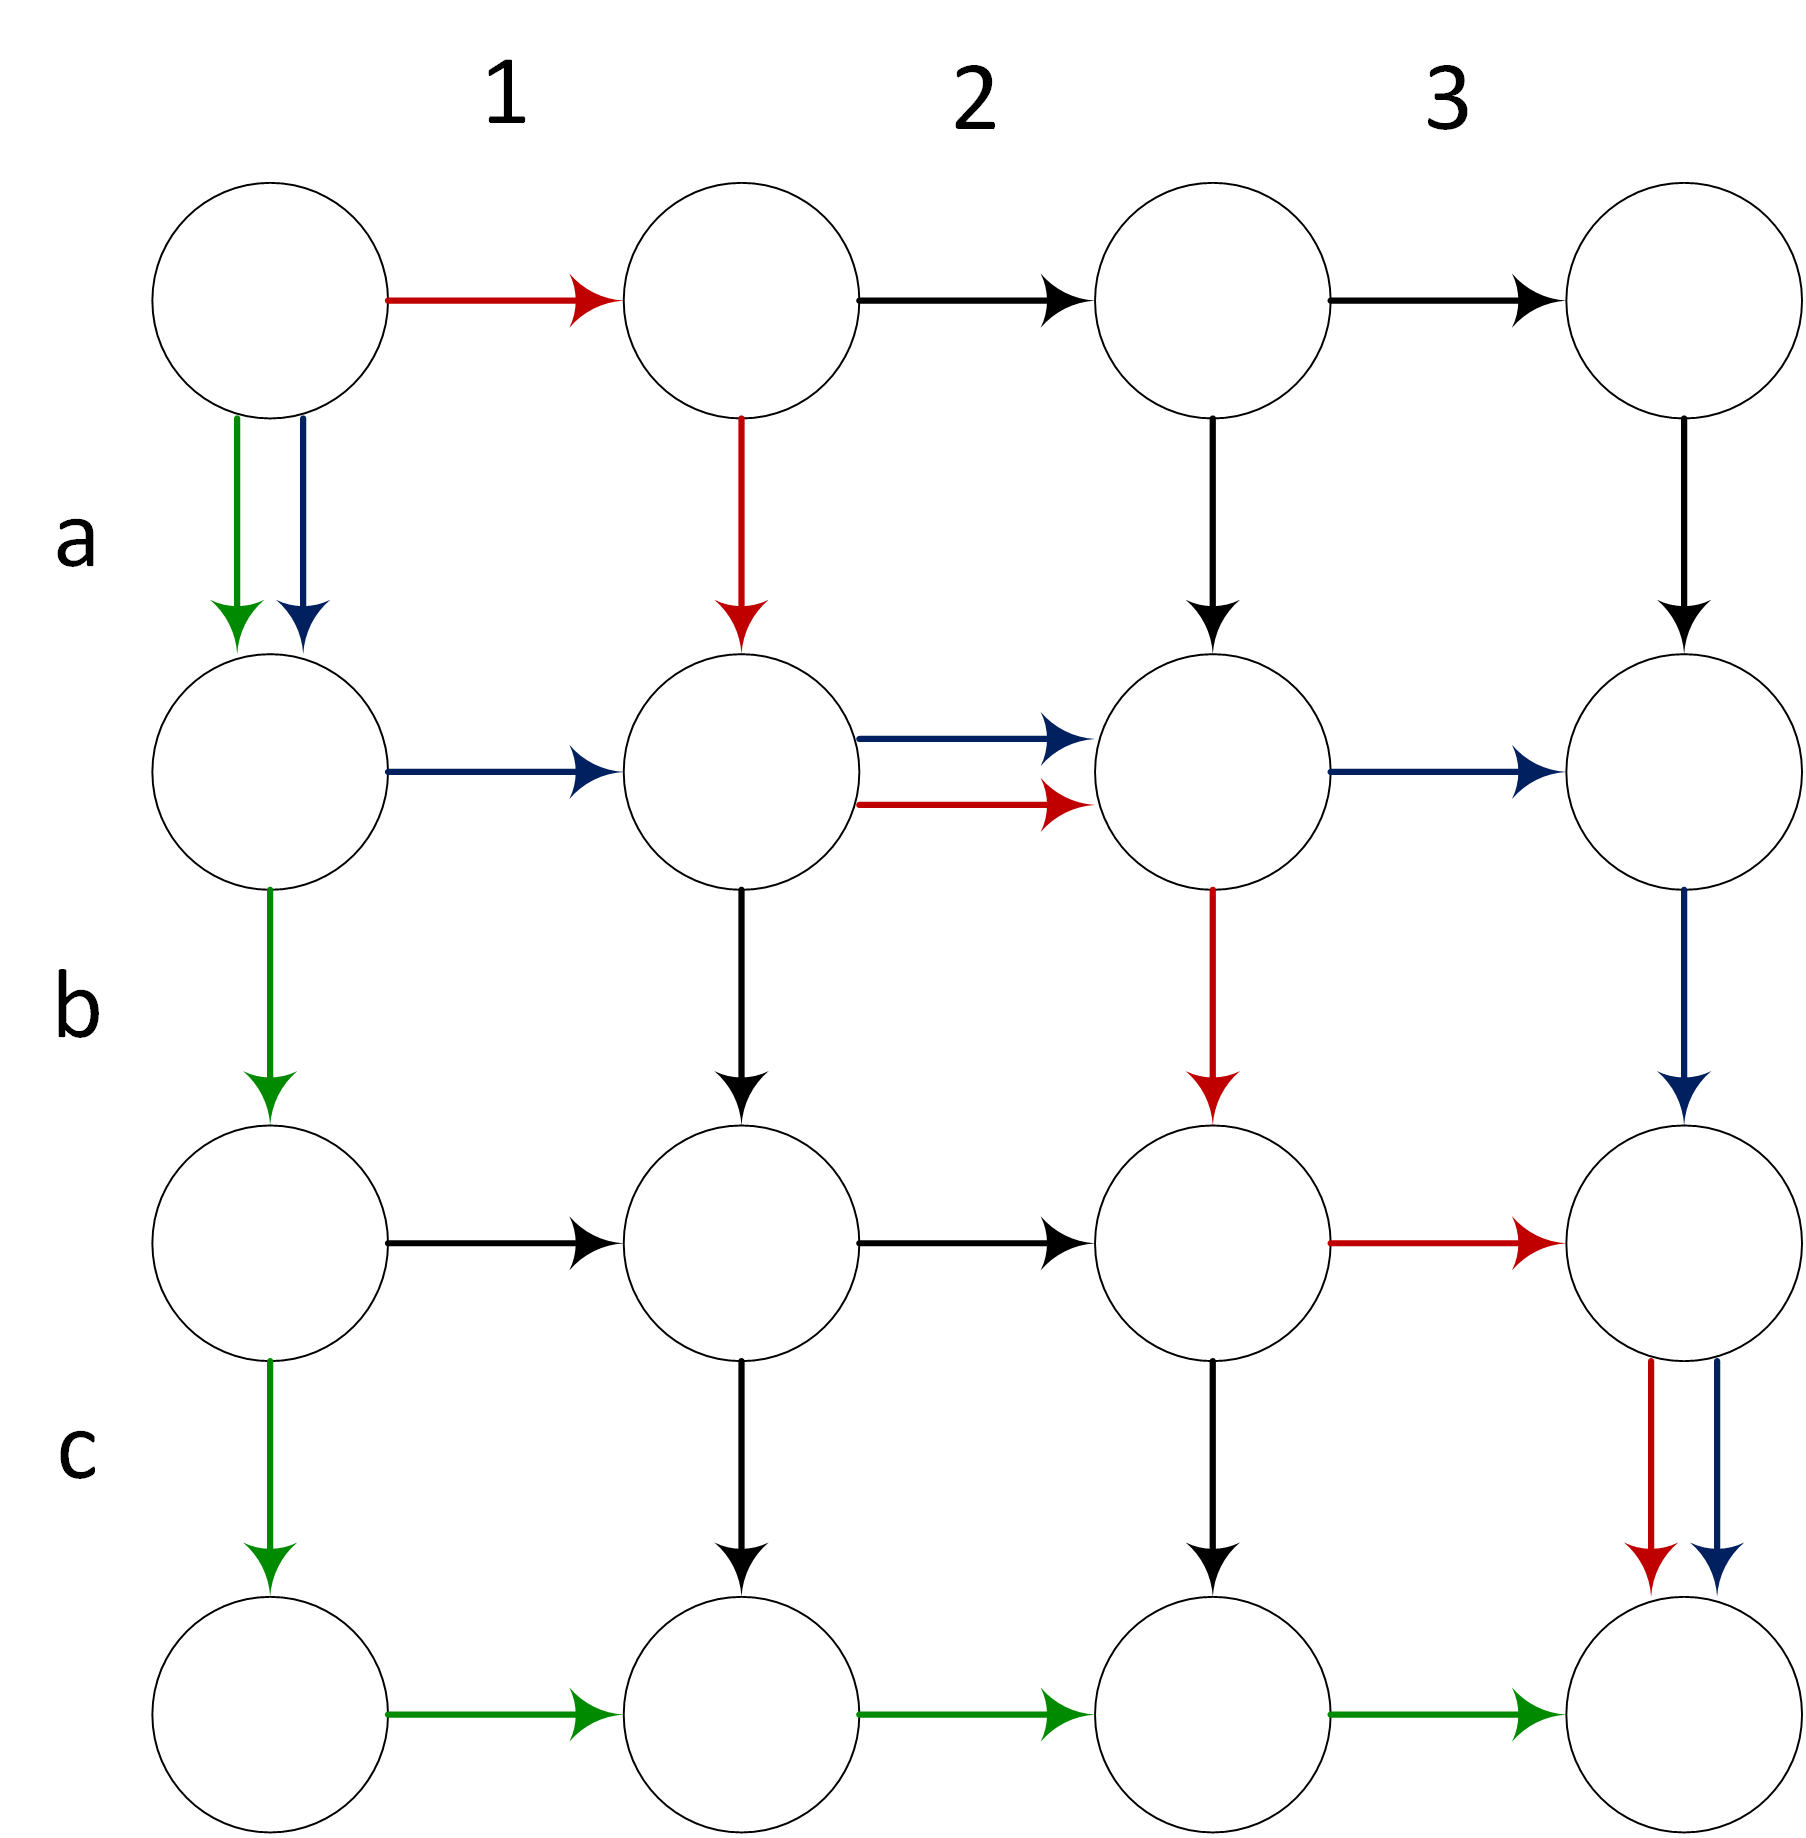
\includegraphics[width=.4\textwidth]{Nondeterminism}\\
\\
Da bei jedem Test der Zeitplaner eine andere Ausführungsreihenfolge (Umstände des Wettrennens, engl. race conditions) wählen kann, ist der Test praktisch nicht reproduzierbar. Wegen der großen Anzahl möglicher Abläufe ist ein systematisches Testen aussichtslos ("`Zustandsexplosion"').

\section{Kritische Bereiche}

\section{Sperren}